\chapter{Entwurf}

Der Ingestion-Prozess ist als erster Schritt im Lebenszyklus der Daten maßgebend für deren Qualität und Aussagekraft bei der späteren Verarbeitung und Analyse \parencite{ingestion_01}.
Daher muss schon bei dem Entwurf nicht nur auf die Anforderungen Rücksicht genommen werden, sondern auch auf das fertige Data-Lake-System.

\section{Architektur}
In dieser Arbeit kann kein komplettes Data-Lake-System entworfen werden.
Es muss jedoch die Entscheidung getroffen werden, nach welcher Architektur das System aufgebaut werden soll.
Damit zuverlässig die Änderungen in einer Datenquelle erkannt werden können, dürfen die Daten, die von der Ingestion geschrieben wurden, nicht direkt verändert werden.
Hierfür ist nur die Zonen-Architektur geeignet, da Daten bei Verlassen des Raw Data Pond aus diesem glöscht werden.
Die Zonen-Architektur kann auch als eine datenorientierte Architektur bezeichnet werden.
Für die Implementierung des Data Lake soll eine Microservice-Architektur zum Einsatz kommen.
Daraus folgt, dass hier ebenfalls eine Aufteilung nach Funktionen der Komponenten notwendig ist.
Daher reicht eine pure datenorientierte Architektur des Data Lake nicht aus.
Am besten eignet sich in diesem Fall die von \textcite{sawadogo2021data} beschriebene hybride Architektur.

\subsection{Zonen-Architektur}
Von \textcite{ingestion_02} wurde eine Architektur basierend auf drei Zonen entwickelt.
\begin{enumerate}
    \item In der \emph{Drop Zone} werden alle Daten ohne weitere Verarbeitung gespeichert.
          Nur die Datenproduzenten haben Zugriff auf diese Zone und können Daten schreiben.
    \item Die \emph{Landing Zone} ist ein unveränderlicher Speicher, der Daten-Assets enthält, die jeweils zu einer Daten-Sammlung gehören. Projekte können mit den Assets aus der Landing Zone interagieren.
          Benutzer müssen lesenden Zugriff auf bestimmte Assets über einen Governance-Prozess beantragen.
    \item Projekte können in der \emph{Integration Zone} angereicherte Daten speichern.
          Diese Anreicherung kann zum Beispiel aus einer Aufarbeitung oder Umstrukturierung bestehen, die speziell für ein Projekt benötigt wird.
          Es ist außerdem möglich Daten aus der Drop Zone wieder in die Landing Zone zu laden.
\end{enumerate}
Zu diesem Zeitpunkt kann noch keine Aussage darüber getroffen werden, ob diese Architektur für die komplette Umsetzung des Data Lake geeignet ist.
Der Ansatz der Drop Zone jedoch, in der nur Datenproduzenten schreiben können, erfüllt genau die Bedingung, dass die Daten der Ingestion nicht durch andere verändert werden dürfen.
Es ist hier wichtig, dass die Daten mit denen neue Daten verglichen werden, seit der letzten Ingestion nicht verändert wurden, um genaue Aussagen über die geschehenen Änderungen in der Datenquelle treffen zu können.
Daher wird zumindest eine Zonen-Architektur mit der Drop Zone für den Entwurf übernommen.
Die Datenproduzenten, in diesem Szenario, sind alle Microservices, die für die Speicherung von Daten zuständig sind.
Die Aufteilung in Funktionen kann ebenfalls noch nicht abgeschlossen werden, da in dieser Arbeit die Ingestion-Schnittstelle nur als die erste Funktion entwickelt wird.
Weitere Funktionen werden erst im Verlauf der Entwicklung hinzugefügt.
Dabei muss aber immer mit überlegt werden, ob neben den Funktionen auch weitere Zonen in der Data-Lake-Architektur hinzugefügt werden.

\subsection{Microservice-Architektur}
\label{sec:arch}

Neben der Architektur des Data Lake muss auch eine Architektur für die Microservices entworfen werden.
Diese legt fest, welche Komponenten benötigt werden, welche Aufgaben sie bearbeiten und wie sie miteinander interagieren.
Der erste Schritt dabei ist es, trennbare Aufgaben zu identifizieren und aufzuteilen.
Der Aufbau der Microservice-Architektur kann entweder funktions- oder prozessorientiert angegangen werden.

Bei einem funktionsorientierten Aufbau wird das System in einzelne Funktionen unterteilt.
Teile dieser Unterteilung können dann einzelnen Microservices zugewiesen werden.
Für die Ingestion-Schnittstelle sind das die Funktionen zum Laden der Daten, für die Deltaberechnung und zur Speicherung der Daten.
Da diese aber ein zusammenhängender Arbeitsablauf sind, der in einem Spark-Job ausgeführt werden kann, sollten diese auch nicht auf verschiedene Microservices aufgeteilt werden.

Hier ist der prozessorientierte Ansatz besser geeignet.
Dabei werden die technischen Abläufe betrachtet, um eine Unterteilung abzuleiten.
Bei der Ingestion-Schnittstelle ergeben sich die API, das kontinuierliche Ausführen und die Ausführung der Ingestion mit Spark.
In \cref{fig:system-architektur} ist die Architektur für die Ingestion-Schnittstelle dargestellt.

Bei dem \textbf{API-Service} handelt es sich um den Service für die Interaktion mit dem Data-Lake-System.
Durch \nameref{ANF_14} ergibt sich, dass dieser ein Web-Server mit einer REST-API ist.
Es geht zwar in dieser Arbeit nur um die Ingestion, aber der API-Service sollte Schnittstellen zu allen Funktionen des Data-Lake-Systems enthalten.

Der \textbf{Ingestion-Service} ist dafür zuständig, die Datenquellen zu verarbeiten und den kompletten Prozess vom Laden bis zum Speichern der Daten in Apache Spark auszuführen.
Die Ingestion soll für eine Datenquelle nur einmal gleichzeitig, aber parallel für unterschiedliche Datenquellen ausgeführt werden können.

Bei einer zeitgesteuerten oder Datenstrom-Ingestion muss die kontinuierliche Ausführung sichergestellt werden.
Das wird durch den \textbf{Continuation-Service} übernommen.
Für alle Datenquellen muss regelmäßig geprüft werden, ob für diese gerade eine Ingestion ausgeführt wird und ausgeführt werden sollte.
Falls keine Ingestion ausgeführt wird, aber ausgeführt werden sollte, wird die Ingestion für diese Datenquelle gestartet.

Neben diesen Mircoservices wird noch ein Nachrichten-Service benötigt.
Der Nachrichten-Service stellt die Kommunikation zwischen den Microservices dar.
Hier ist es wichtig, dass es einem Sender möglich ist, Nachrichten an einen oder auch an mehrere Empfänger zu senden.
So soll sichergestellt werden, dass bestehende Microservices einfach repliziert und neue eingefügt werden können.
Für das Speichern von Daten und Metadaten wird jeweils ein Speichersystem benötigt.

\begin{figure}
    \centering
    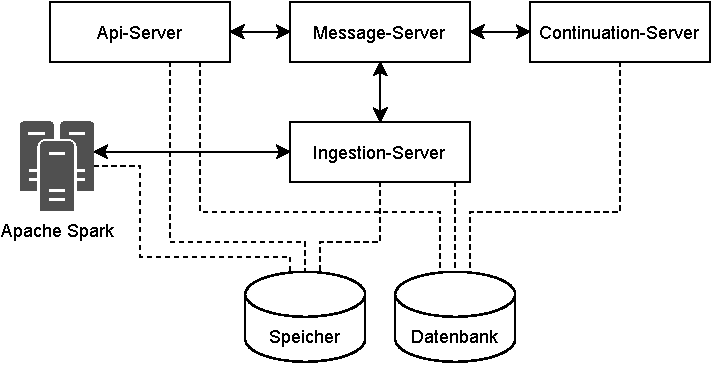
\includegraphics{Grafiken/Entwicklung-System-Architektur.pdf}
    \caption{Microservice-Architektur der Ingestion}
    \label{fig:system-architektur}
\end{figure}

\section{Plugins}

In \ref{ANF_04} wird durch ANF\_04 gefordert, dass zusätzlicher Code bei der Ingestion ausgeführt werden können soll.
Das soll durch Plugins umgesetzt werden.
Die Plugins werden jeder Datenquelle einzeln hinzugefügt und werden an verschiedenen, fest definierten Punkten der Ingestion ausgeführt. 
Da die Plugins eventuell auf Software-Bibliotheken zurückgreifen müssen, die nicht auf dem Data-Lake-System vorhanden sind, kann zusätzlich eine Liste von Abhängigkeiten der Plugins angegeben werden.

Bei der Ingestion gibt es zwei Stellen, an denen das Einbringen eines Plugins sinnvoll sein kann.
Die erste ist zum Laden der Daten als Load-Plugin.
Hier wird das standardmäßige Vorgehen der Ingestion mit dem des Plugins ersetzt.
Dadurch wird es möglich anders als nur über \textit{Apache Spark} Daten zu laden.
Ein Beispiel dafür ist die Verwendung einer REST-API als Datenquelle.
Das Plugin kann erst über mehrere Abfragen der REST-API den Datensatz abholen und diesen dann erst in eine DataFrame umwandeln.
Ein Load-Plugin muss immer eine DataFrame zurück geben, mit dem danach in der Ingestion weiter verfahren werden kann.
Damit ein DataFrame erstellt werden kann,  muss dem Plugin außerdem die entsprechende SparkSession mitgegeben werden.

Das After-Load-Plugin setzt im Gegensatz direkt nach dem Laden der Daten an.
Diesem Plugin wird das geladene DataFrame übergeben und es muss auch wieder ein DataFrame zurück geben.
Es kann genutzt werden um vor dem Speichern der Daten kleinere Anpassungen am Datensatz zu machen.
\section{Metadatenmodell}

Wie bereits erwähnt muss ein Modell erstellt werden, dass die Metadaten abbildet, die bei einer Ingestion erfasst werden (\cref{fig:datenmodell}).
Zu diesen Metadaten gehören alle Informationen über die Herkunft der Daten, also die Datenquelle und das Speicherziel.
Diese werden zum Großteil in für Spark erforderlichen Parametern widergespiegelt.
Ein weiterer Teil der Metadaten sind alle Informationen über die Ausführung einer Ingestion.

\subsection{DatasourceDefinition}

Das Metadatenmodell beschreibt eine Datenquelle und hat als zentrales Element das Konzept DatasourceDefinition.
Ein Teil des Modells besteht aus Feldern, die für Spark erforderlichen Informationen enthalten.
Dazu gehören: \begin{itemize}
    \item zusätzliche Abhängigkeiten für Spark (spark.jars.packages),
    \item das Format und Optionen für die Reader und
    \item bei benutzerdefinierten Speichersystemen das Format, die Optionen und einen Schreibmodus für die Writer.
\end{itemize}
Neben den Spark spezifischen werden noch folgende weitere Informationen erfasst: \begin{itemize}
    \item ein Name für die Datenquelle,
    \item die Id einer anderen Datenquelle, falls die aktuelle eine Update-Quelle ist,
    \item das Datum der Erstellung und letzten Änderung,
    \item den Namen der Id-Spalte in den Daten (wird später für die Deltaberechnung benötigt),
    \item den Typ, der zu lesenden Daten,
    \item eine Liste der zu laden Dateien, wenn es sich um eine Datei-Ingestion handelt,
    \item den Typ, wie die Daten geschrieben werden müssen,
    \item eine Liste mit der Zeitsteuerung für eine kontinuierliche Ingestion,
    \item eine Liste mit Plugindateien und
    \item eine Liste mit Abhängigkeiten der Plugins.
\end{itemize}

Die möglichen Lese-Typen ergeben sich aus der Betrachtung, wie die Daten in das Data-Lake-System gelangen und welche Struktur sie haben.
Bei einer Pull-Ingestion ist das System dafür verantwortlich Daten aus einer Quelle zu laden.
Dies ist zum Beispiel bei Datenbanken der Fall.
Das Gegenteil dazu ist eine Push-Ingestion, bei der die Daten direkt an den Data Lake gesendet werden.
Diese muss jedoch nochmal in zwei unterschiedliche Typen unterteilt werden.
Bei einer Stream-Ingestion, also bei Datenströmen, werden kontinuierlich neue Daten an das System gesendet.
Und bei einer File-Ingestion werden Dateien hochgeladen, die die Daten enthalten, wobei wichtig ist, dass alle Dateien das gleiche Dateiformat und je nach Typ eine ähnliche oder gleiche Struktur haben.
Die Dateien können sich in Daten- und Quelldateien unterscheiden.
Datendateien enthalten unstrukturierte Daten und werden einfach im HDFS mit abgelegt, ohne weiter verarbeitet zu werden.
Das könnten zum Beispiel Bilder oder Videos sein.
Quelldateien enthalten mindestens semistrukturierte Daten und dienen dem Zweck, in ein anderes Speicherformat, wie zum Beispiel Parquet oder eine Delta-Tabelle geschrieben zu werden.
Es ist nicht möglich, Daten direkt an die API zu senden.
Alle Push-Ingestions sollen über diese beiden Typen abgebildet werden.

Die möglichen Schreib-Typen werden aus den Speicherzielen abgeleitet.
Custom bedeutet, dass der in der DatasourceDefinition konfigurierte Speicher verwendet werden soll.
Delta ist das Speichern im internen Speicher aber mit einer Versionierung und Default ist das Speichern ohne Versionierung.

Für die Umsetzung einer unkomplizierten Versionierung der DatasourceDefinition werden alle veränderlichen Informationen in Revisionen gespeichert.
Das betrifft alle oben genannten Felder.
Die Revisionen einer DatasourceDefinition erhalten eine fortlaufende Nummer.
Die DatasourceDefinition selbst hält dann nur noch eine Liste aller Revisionen und die Nummer der aktuellen.

\subsection{IngestionEvent}

Das Modell für den Ablauf einer Ingestion ist das IngestionEvent.
Dieses enthält, wie die Revision, eine fortlaufende Nummer, ein Start- und Enddatum, den aktuellen Status indem es sich befindet, die Nummer der Revision mit der es gestartet wurde und eine Fehlernachricht, falls ein Fehler aufgetreten ist.

Das IngestionEvent kann auch zur DatasourceDefinition hinzugefügt werden.
Dafür werden Felder hinzugefügt, die alle IngestionEvents, die Nummer des letzten und die Nummer des letzten erfolgreichen IngestionEvents enthalten.

\begin{figure}
    \centering
    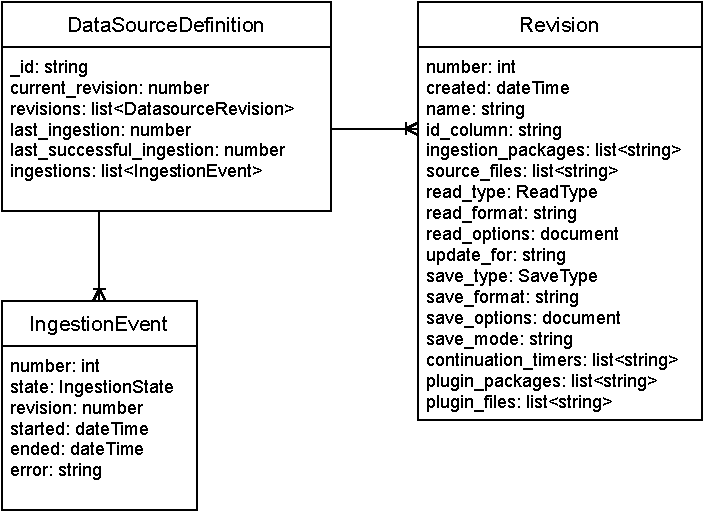
\includegraphics{Grafiken/Entwicklung-Datenmodell.pdf}
    \caption{Übersicht Metadatenmodell}
    \label{fig:datenmodell}
\end{figure}
\section{API-Service}

Für den API-Service müssen Endpunkte definiert werden.
Diese Endpunkte bilden die verschiedenen Funktionen ab, die auf der Ingestion-Schnittstelle ausgeführt werden können.
Dazu gehören die Verwaltung von Datenquellen und das Starten einer Ingestion.
Da es bereits festgelegt wurde, dass es sich um eine REST-Schnittstelle handelt, werden Endpunkte durch einen Pfad und eine HTTP-Methode definiert.
Nachfolgend werden alle Endpunkte aufgelistet.

\begin{table}[ht]
  \centering
  \begin{tabularx}{\linewidth}{lX}
    GET & /datasources \\
    \multicolumn{2}{l}{Liefert alle im System gespeicherten Datenquellen} \\
    \\
    GET & /datasources/\textless id\textgreater \\
    \multicolumn{2}{l}{Liefert die Datenquelle mit der im Pfad übergebenen Id} \\
    \\
    POST & /datasources \\
    \multicolumn{2}{l}{Bearbeitet die Daten Datenquelle mit der im Pfad übergebenen Id} \\
    \\
    PUT &  /datasources/\textless id\textgreater \\
    \multicolumn{2}{l}{Erstellt eine neue Datenquelle} \\
    \\
    GET &  /datasources/\textless id\textgreater/run \\
    \multicolumn{2}{l}{Startet eine Ingestion der Datenquelle mit der im Pfad übergebenen Id}
    
    
    
    %\hline
    %Pfad                                      & HTTP-Methode & Beschreibung                                                          \\
    %\hline \hline
    %/datasources                              & GET          & Liefert alle im System gespeicherten Datenquellen                     \\
    %\hline
    %/datasources/\textless id\textgreater     & GET          & Liefert die Datenquelle mit der im Pfad übergebenen Id                \\
    %\hline
    %/datasources                              & POST         & Erstellt eine neue Datenquelle                                        \\
    %\hline
    %/datasources/\textless id\textgreater     & PUT          & Bearbeitet die Daten Datenquelle mit der im Pfad übergebenen Id       \\
    %\hline
    %/datasources/\textless id\textgreater/run & GET          & Startet eine Ingestion der Datenquelle mit der im Pfad übergebenen Id \\
    %\hline
  \end{tabularx}
  %\caption{Endpunkte des API-Servers}
  \label{tab:enpoints}
\end{table}

Außerdem kümmert sich der API-Service um die Erstellung von Datenquellen, deren Revisionen und Ingestion-Events.
Bei Anfragen zum Starten einer Ingestion versendet der API-Server eine Nachricht, mit der Id der Datenquelle.
\section{Continuation-Service}

Für die Sicherstellung der korrekten Ausführung kontinuierlicher Ingestions, müssen regelmäßig alle Datenquellen überprüft werden.
Dabei gibt es zwei Bedingungen nach denen entscheiden wird, ob eine Ingestion werden muss.
Bei Datenströmen gilt allgemein, wenn dieser nicht läuft, dann muss die Ingestion automatisch neu gestartet werden.
Eine Ausnahme dabei ist, wenn die Verarbeitung durch den Benutzer explizit beendet wurde.

Der zweite Fall ist die Zeitsteuerung.
Für eine zeitgesteuerte kontinuierliche Ingestion werden einer Datenquelle ein oder mehrere Timer hinzugefügt.
Der Continuation-Service prüft, ob der Timer zu diesem Zeitpunkt zutrifft oder nicht.
Wenn das der Fall ist und bisher keine Ingestion auf der Datenquelle läuft, dann wird eine neue gestartet.

In Unix-Systemen gibt es bereits eine Lösung für die Notation solcher Timer.
Dort gibt es die sogenannten Cron-Jobs, mit deren Hilfe Aufgaben automatisch und regelmäßig ausgeführt werden können.
Dabei wird der Zeitpunkt der Ausführung über fünf Felder festgelegt.
Diese geben die Minute, die Stunde, den Tag des Monats, den Monat und den Tag der Woche als Zahlen an.
Als Erweiterung kann man "`*"' als Platzhalter für alle möglichen Werte verwenden, man kann mehrere Werte als mit Kommata getrennt angeben oder mit "`/x"' eine Liste in Schritten der Größe $x$ erzeugen \parencite{cron}.

Diese Notation soll auch für die Zeitsteuerung der Ingestions genutzt werden.
Als Referenz wird dabei die koordinierte Weltzeit (UTC) genommen, damit die Ausführung unabhängig vom Standort einheitlich bleibt.
Wenn eine Datenquelle mehrere Timer hat, reicht es aus, dass einer von diesen zutrifft.
\section{Ingestion-Service}
\label{sec:entw-ingestion}

Der Ingestion-Service hat die Aufgabe den Spark-Job für die Ausführung einer Ingestion zu erstellen, zu starten, zu überwachen und den Status des IngestionEvents anzupassen.
Dazu gehört das Festlegen des Ablaufs zum Laden der Daten in ein DataFrame, zur Deltaberechnung und zum Speichern.
Ein zweiter wichtiger Teil ist die Integration der Plugins in den Ingestion-Prozess.
Ebenfalls koordiniert der Ingestion-Service die parallele Ausführung von Ingestions.

Der Ingestion-Service wartet auf die Nachricht zur Ausführung einer Ingestion, mit der Id der DatasourceDefinition.
Als erstes wird geprüft, ob bereits eine Ingestion der Datenquelle aktiv ist.
Falls das nicht der Fall ist, wird ein neuer Prozess gestartet, indem die Ingestion ausgeführt wird.
Auf diese Art wird die Parallelität ermöglicht.

Der Ablauf einer Ingestion kann unabhängig vom Lese- und Schreib-Typ in einem allgemeinen Ablauf, wie in \cref{fig:ingestion-ablauf}, abgebildet werden.
Als erstes wird die Ingestion vorbereitet.
Hier werden die Plugins und deren Abhängigkeiten installiert und eine SparkSession erstellt.
Im nächsten Schritt werden die Daten aus der Quelle geladen.
Wenn es sich dabei um Änderungsdaten aus einer Update-Quelle handelt, können diese direkt in den entsprechenden Zieldatensatz eingepflegt werden.
Ist das nicht der Fall, folgt eine Entscheidung, ob Änderungsdaten berechnet werden müssen.
Es gelten die folgenden zwei Regeln: \begin{itemize}
    \item der Speicher-Typ ist Delta und
    \item es ist nicht die erste Ingestion dieser Datenquelle.
\end{itemize}
Wurden Änderungsdaten berechnet, werden diese eingepflegt.
Wurden keine berechnet, werden die Daten einfach gespeichert.
Ist das Speicherziel dabei ein Delta-Tabelle wird diese angelegt und ist es eine Parquet-Datei, dann werden die aktuellen Daten überschrieben.
Handelt es sich nicht um einen benutzerdefinierten Speicher, werden die alten Daten mit den neuen überschrieben.

\begin{figure}
    \centering
    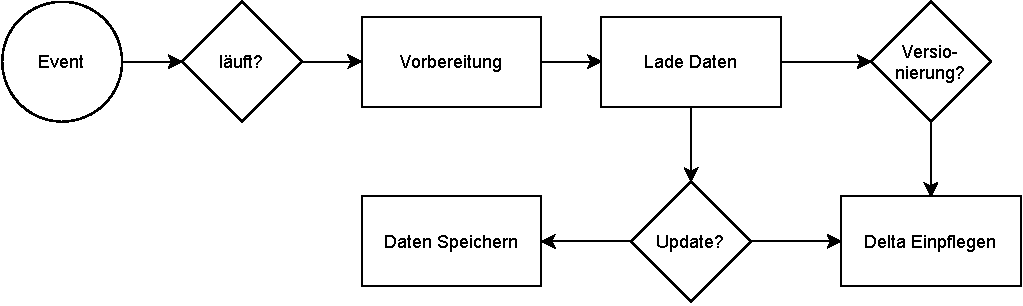
\includegraphics[width=\textwidth]{Grafiken/Entwicklung-Ingestion-Ablauf.pdf}
    \caption{Ablauf einer Ingestion}
    \label{fig:ingestion-ablauf}
\end{figure}